\documentclass[conference]{IEEEtran}
\IEEEoverridecommandlockouts
\usepackage[utf8]{inputenc}
\usepackage[T1]{fontenc}
\usepackage[brazil]{babel}
\usepackage{amsmath,amssymb}
\usepackage{graphicx}
\usepackage{url}
\usepackage{xcolor}
\usepackage{microtype}
\newcommand{\nRatings}{100.000}
\newcommand{\nUsers}{943}
\newcommand{\nItems}{1.682}
\newcommand{\density}{6,30}
\newcommand{\emptyShare}{93,7}
\newcommand{\meanRating}{3,53}
\newcommand{\stdRating}{1,13}
\newcommand{\rpuMin}{20}
\newcommand{\rpuMed}{65}
\newcommand{\rpuMean}{106}
\newcommand{\rpuMax}{737}
\newcommand{\rpiMed}{27}
\newcommand{\rpiMean}{59}
\newcommand{\rpiMax}{583}
\newcommand{\itemsLtTen}{32}
\newcommand{\topTwentyShare}{65}
\newcommand{\bestSim}{Pearson}
\newcommand{\bestMode}{centralizado}
\newcommand{\bestRMSE}{0,948}
\newcommand{\bestRMSEstd}{0,007}
\newcommand{\bestMAE}{0,742}
\newcommand{\bestK}{80}
\newcommand{\winsGlobal}{5}
\newcommand{\winsUser}{5}
\newcommand{\winsItem}{5}
\newcommand{\nFolds}{5}
\newcommand{\baseGlobal}{1,126}
\newcommand{\baseUser}{1,044}
\newcommand{\baseItem}{1,025}
\newcommand{\gainItemPct}{7,5}
\newcommand{\gainUserPct}{9,2}
\newcommand{\gainGlobalPct}{15,8}
\newcommand{\runtime}{2}

\newcommand{\exUser}{54}
\newcommand{\exN}{65}
\newcommand{\exK}{80}

\AtBeginDocument{\renewcommand{\figurename}{Fig.}}
\setlength{\tabcolsep}{3pt}

\begin{document}

\title{Recomenda\c{c}\~ao de Filmes por Filtragem Colaborativa Baseada em Usu\'arios com KNN: Uma Avalia\c{c}\~ao no MovieLens 100K}

\author{\IEEEauthorblockN{[Nome do Integrante 1]}
\IEEEauthorblockA{{[Curso]}\\
{[Institui\c{c}\~ao], [Cidade/UF]}\\
{[e-mail]}}
\and
\IEEEauthorblockN{[Nome do Integrante 2]}
\IEEEauthorblockA{{[Curso]}\\
{[Institui\c{c}\~ao], [Cidade/UF]}\\
{[e-mail]}}
\and
\IEEEauthorblockN{[Nome do Integrante 3]}
\IEEEauthorblockA{{[Curso]}\\
{[Institui\c{c}\~ao], [Cidade/UF]}\\
{[e-mail]}}}

\maketitle

\begin{abstract}
Este trabalho avalia a filtragem colaborativa baseada em usuários com k-vizinhos mais próximos (KNN) no conjunto MovieLens 100K, que reúne 100.000 avaliações de 943 usuários sobre 1.682 filmes. Foram comparadas três similaridades (cosseno, Pearson e diferença quadrática média, MSD), com e sem centralização das notas, em validação cruzada de 5 partições e com o número de vizinhos escolhido apenas com dados de treino. A melhor configuração, Pearson com notas centralizadas (empatada com a MSD centralizada), atingiu RMSE de 0,948 e MAE de 0,742, valor 7,5\% menor que o da média por filme, e superou os três baselines em todas as partições. A centralização das notas teve mais efeito que a escolha da similaridade, e a hipótese de que Pearson e cosseno superariam a medida baseada em distância euclidiana foi refutada. Nas listas com os 10 filmes recomendados, o KNN (Precision@10 de 0,093, exigindo ao menos 20 vizinhos) ficou abaixo da lista dos filmes mais populares (0,157), e o erro de previsão diminuiu com o histórico do usuário (RMSE de 1,024 para 0,925 entre os grupos extremos).
\end{abstract}

\begin{IEEEkeywords}
filtragem colaborativa, k-vizinhos mais pr\'oximos, MovieLens, sistemas de recomenda\c{c}\~ao, similaridade de Pearson
\end{IEEEkeywords}

\vspace{3pt}
\noindent{\footnotesize\textbf{\textit{Abstract}---This paper evaluates user-based collaborative filtering with k-nearest neighbors (KNN) on the MovieLens 100K dataset (100,000 ratings from 943 users on 1,682 movies). Three similarity measures (cosine, Pearson and mean squared difference) were compared, with and without mean-centering of the ratings, using 5-fold cross-validation and choosing the number of neighbors with training data only. Pearson with centered ratings, tied with centered MSD, reached an RMSE of 0.948 (MAE 0.742), 7.5\% below the per-movie mean baseline, and beat all three baselines in every fold. Centering mattered more than the choice of similarity, and the hypothesis that Pearson and cosine would outperform the Euclidean-based measure was refuted. In top-10 lists, KNN (Precision@10 of 0.093 with at least 20 neighbors) fell short of a most-popular list (0.157), while prediction error decreased as users had more ratings (RMSE from 1.024 to 0.925 between the extreme groups).}}


%=====================================================================
\section{Introdu\c{c}\~ao}
Plataformas de v\'ideo e de filmes oferecem cat\'alogos com milhares de t\'itulos. Diante de tantas op\c{c}\~oes, o usu\'ario gasta tempo escolhendo e pode desistir sem encontrar algo de que goste. Sistemas de recomenda\c{c}\~ao reduzem esse esfor\c{c}o ao sugerir t\'itulos adequados a cada pessoa. Entre as t\'ecnicas dispon\'iveis, a filtragem colaborativa \'e uma das mais cl\'assicas: ela usa apenas o hist\'orico de avalia\c{c}\~oes dos usu\'arios, sem precisar conhecer o conte\'udo dos filmes \cite{resnick1994,desrosiers2011}.

O desafio central \'e a esparsidade. Cada usu\'ario avalia somente uma pequena fra\c{c}\~ao do cat\'alogo, de modo que a maior parte das notas \'e desconhecida. \'E preciso estimar a nota que um usu\'ario daria a filmes que ainda n\~ao viu e, a partir dessas estimativas, ordenar os filmes para montar uma lista de sugest\~oes. Na filtragem colaborativa baseada em usu\'arios, parte-se da ideia de que pessoas que avaliaram de modo parecido no passado tendem a concordar no futuro. Assim, para recomendar a um usu\'ario, buscam-se seus $k$ vizinhos mais parecidos (KNN) e aproveitam-se as notas deles \cite{resnick1994,herlocker1999}.

Este trabalho implementa e avalia esse m\'etodo no conjunto de dados MovieLens 100K \cite{harper2015}. A pergunta de pesquisa que orienta o estudo \'e:

\begin{quote}
\textit{Em que medida as avalia\c{c}\~oes de usu\'arios com gostos semelhantes permitem recomendar filmes que um usu\'ario avaliaria bem?}
\end{quote}

Essa pergunta \'e desdobrada em quatro perguntas espec\'ificas, cada uma com uma hip\'otese a ser confirmada ou refutada pelos experimentos:

\begin{itemize}
\item \textbf{PE1.} Qual medida de similaridade entre usu\'arios (cosseno, correla\c{c}\~ao de Pearson ou diferen\c{c}a quadr\'atica m\'edia) gera as melhores previs\~oes? \textit{H1:} Pearson e cosseno superam a medida baseada em dist\^ancia euclidiana, que sofre mais com a esparsidade.
\item \textbf{PE2.} Qual n\'umero de vizinhos $k$ equilibra precis\~ao e generaliza\c{c}\~ao, e centralizar as notas pela m\'edia de cada usu\'ario ajuda? \textit{H2:} existe um $k$ intermedi\'ario \'otimo, e a centraliza\c{c}\~ao reduz o erro, pois alguns usu\'arios avaliam sempre mais alto ou mais baixo que os demais.
\item \textbf{PE3.} O KNN prev\^e as notas melhor do que baselines simples (m\'edia global, do filme e do usu\'ario)? \textit{H3:} sim, mas a vantagem sobre a m\'edia do filme \'e modesta.
\item \textbf{PE4.} As listas de $N$ filmes recomendados acertam o que o usu\'ario de fato gostou, e como a esparsidade afeta o resultado? \textit{H4:} usu\'arios com mais avalia\c{c}\~oes recebem recomenda\c{c}\~oes melhores do que os que t\^em poucas.
\end{itemize}

As contribui\c{c}\~oes s\~ao: (i) uma compara\c{c}\~ao controlada de tr\^es similaridades, com e sem centraliza\c{c}\~ao das notas; (ii) uma sele\c{c}\~ao de hiperpar\^ametros feita apenas com dados de treino; (iii) a avalia\c{c}\~ao tanto da previs\~ao de notas quanto das listas de recomenda\c{c}\~ao; e (iv) uma an\'alise por grupos de usu\'arios segundo o volume de avalia\c{c}\~oes. O c\'odigo e os scripts para reproduzir todas as tabelas e figuras est\~ao em \url{https://github.com/[usuario]/[repositorio]}.

O restante do artigo est\'a organizado assim: a Se\c{c}\~ao~II apresenta os modelos e a justificativa de cada um; a Se\c{c}\~ao~III descreve o conjunto de dados; a Se\c{c}\~ao~IV detalha como os experimentos foram feitos; a Se\c{c}\~ao~V traz os resultados e a discuss\~ao; e a Se\c{c}\~ao~VI conclui.

%=====================================================================
\section{Fundamenta\c{c}\~ao e Modelos}
\subsection{Filtragem colaborativa baseada em usu\'arios}
Seja $r_{ui}$ a nota do usu\'ario $u$ ao filme $i$ e $\bar{r}_u$ a m\'edia das notas de $u$. Para prever $\hat{r}_{ui}$, considera-se o conjunto $N_k(u,i)$ dos $k$ usu\'arios mais similares a $u$ entre os que avaliaram $i$ e cuja similaridade $s(u,v)$ \'e positiva. No modelo \emph{b\'asico}, a previs\~ao \'e a m\'edia das notas dos vizinhos ponderada pela similaridade:
\begin{equation}
\hat{r}_{ui}=\frac{\sum_{v\in N_k(u,i)} s(u,v)\, r_{vi}}{\sum_{v\in N_k(u,i)} s(u,v)}.
\end{equation}
No modelo \emph{centralizado}, trabalha-se com o desvio da nota de cada vizinho em rela\c{c}\~ao \`a m\'edia dele e soma-se de volta a m\'edia do usu\'ario alvo \cite{herlocker1999}:
\begin{equation}
\hat{r}_{ui}=\bar{r}_u+\frac{\sum_{v\in N_k(u,i)} s(u,v)\,(r_{vi}-\bar{r}_v)}{\sum_{v\in N_k(u,i)} s(u,v)}.
\end{equation}
A centraliza\c{c}\~ao foi inclu\'ida para corrigir o fato de que alguns usu\'arios d\~ao quase sempre notas altas e outros, notas baixas. Quando $N_k(u,i)$ \'e vazio, a previs\~ao \'e $\bar{r}_u$, e o resultado \'e limitado ao intervalo $[1,5]$. O KNN usu\'ario-usu\'ario foi escolhido por ser simples, interpret\'avel (\'e poss\'ivel mostrar quais usu\'arios influenciaram uma recomenda\c{c}\~ao) e por ser o ponto de partida cl\'assico da \'area.

\subsection{Medidas de similaridade}
Seja $I_{uv}$ o conjunto de filmes avaliados por ambos os usu\'arios. Tr\^es medidas foram comparadas, todas calculadas somente sobre $I_{uv}$ e iguais a zero quando $|I_{uv}|$ \'e menor que um suporte m\'inimo (Se\c{c}\~ao~IV):
\begin{align}
s_{\cos}(u,v)&=\frac{\sum_{i\in I_{uv}} r_{ui}r_{vi}}{\sqrt{\sum_{i\in I_{uv}} r_{ui}^2}\sqrt{\sum_{i\in I_{uv}} r_{vi}^2}},\\
s_{\mathrm{pear}}(u,v)&=\frac{\sum_{i\in I_{uv}}(r_{ui}-\mu_u)(r_{vi}-\mu_v)}{\sqrt{\sum_{i\in I_{uv}}(r_{ui}-\mu_u)^2}\sqrt{\sum_{i\in I_{uv}}(r_{vi}-\mu_v)^2}},\\
s_{\mathrm{msd}}(u,v)&=\frac{1}{1+\frac{1}{|I_{uv}|}\sum_{i\in I_{uv}}(r_{ui}-r_{vi})^2},
\end{align}
em que $\mu_u$ e $\mu_v$ s\~ao as m\'edias das notas de $u$ e $v$ sobre $I_{uv}$. O cosseno mede o \^angulo entre os vetores de notas. A correla\c{c}\~ao de Pearson olha o padr\~ao das notas e n\~ao o valor absoluto, de modo que dois usu\'arios que preferem os mesmos filmes s\~ao considerados parecidos mesmo que um seja mais exigente que o outro. A medida MSD (\emph{mean squared difference}) \'e a similaridade derivada da dist\^ancia euclidiana, como em \cite{hug2020}, e valoriza notas num\'ericamente pr\'oximas.

\subsection{Baselines}
Tr\^es preditores simples servem de refer\^encia m\'inima: a m\'edia global de todas as notas de treino, a m\'edia de cada usu\'ario e a m\'edia de cada filme (com a m\'edia global quando o filme n\~ao aparece no treino). Um sistema de recomenda\c{c}\~ao s\'o \'e \'util se superar esses valores. Na tarefa de listas de recomenda\c{c}\~ao, as refer\^encias s\~ao a lista dos filmes mais populares (mais avaliados no treino) e a lista dos filmes de maior nota m\'edia entre os que t\^em ao menos 20 avalia\c{c}\~oes.

\subsection{Modelos n\~ao implementados}
O KNN item-item \cite{sarwar2001} e m\'etodos de fatora\c{c}\~ao matricial s\~ao alternativas conhecidas, mas ficam fora do escopo deste trabalho e s\~ao indicados como trabalhos futuros.

%=====================================================================
\section{Conjunto de Dados}
Foi usado o MovieLens 100K, mantido pelo grupo GroupLens Research, da Universidade de Minnesota \cite{harper2015,grouplens}. Ele cont\'em \nRatings{} avalia\c{c}\~oes de 1 a 5 feitas por \nUsers{} usu\'arios sobre \nItems{} filmes, coletadas pelo site MovieLens entre setembro de 1997 e abril de 1998. Cada usu\'ario avaliou ao menos 20 filmes. Foram utilizados o arquivo de notas (\texttt{u.data}), o arquivo de filmes (\texttt{u.item}, para t\'itulos e g\^eneros nos exemplos) e as cinco divis\~oes 80/20 que acompanham o conjunto (\texttt{u1} a \texttt{u5}). Os dados demogr\'aficos (\texttt{u.user}) n\~ao foram usados, pois o modelo depende apenas das notas.

A Fig.~\ref{fig:dataset}(a) mostra que as notas se concentram nos valores altos: a nota 4 é a mais frequente (34,2\%), seguida das notas 3 (27,1\%) e 5 (21,2\%); a nota média é \meanRating{} (desvio padrão \stdRating{}). A matriz usuário-filme tem densidade de apenas \density\%, ou seja, \emptyShare\% das células estão vazias. O número de notas por usuário varia de \rpuMin{} a \rpuMax{}, com mediana \rpuMed{} e média \rpuMean{}; por filme, a mediana é \rpiMed{} (média \rpiMean{}, máximo \rpiMax{}). A distribuição tem cauda longa (Fig.~\ref{fig:dataset}(b)): \itemsLtTen\% dos filmes têm menos de 10 avaliações, enquanto os 20\% de filmes mais avaliados concentram \topTwentyShare\% de todas as notas.

\begin{figure}[t]
\centering
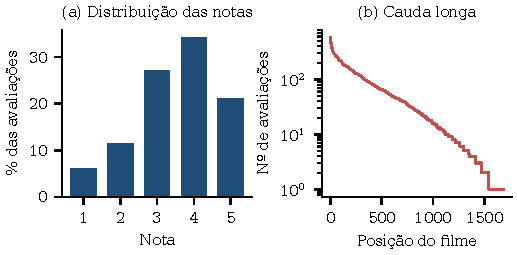
\includegraphics[width=\columnwidth]{assets/figs/fig_dataset.pdf}
\caption{Conjunto MovieLens 100K: (a) distribuição das notas; (b) número de avaliações por filme, com os filmes em ordem decrescente de popularidade (eixo vertical em escala logarítmica).}
\label{fig:dataset}
\end{figure}

O uso \'e livre para pesquisa, com a condi\c{c}\~ao de citar o artigo que descreve o conjunto \cite{harper2015}; uso comercial e redistribui\c{c}\~ao dependem de autoriza\c{c}\~ao. Por isso o reposit\'orio do projeto n\~ao inclui os arquivos de dados e traz apenas instru\c{c}\~oes para baix\'a-los da fonte oficial. Duas limita\c{c}\~oes devem ser lembradas: os dados s\~ao de 1997 e 1998, ent\~ao os resultados mostram o comportamento do m\'etodo e n\~ao o gosto atual do p\'ublico; e como todo usu\'ario tem ao menos 20 notas, o problema do usu\'ario novo (\emph{cold start}) n\~ao \'e avaliado.

%=====================================================================
\section{Metodologia Experimental}
\subsection{Protocolo de valida\c{c}\~ao}
Os experimentos usam a valida\c{c}\~ao cruzada de 5 partes fornecida com o conjunto: em cada uma das divis\~oes \texttt{u1} a \texttt{u5}, 80\% das avalia\c{c}\~oes formam o treino e 20\% formam o teste, e os cinco conjuntos de teste n\~ao se sobrep\~oem. As divis\~oes n\~ao s\~ao estratificadas por usu\'ario: o n\'umero de usu\'arios com ao menos um filme relevante no teste varia de 456 a 890 entre as partes. Os resultados s\~ao reportados como m\'edia e desvio padr\~ao amostral sobre as cinco divis\~oes.

\subsection{Sele\c{c}\~ao de hiperpar\^ametros}
O n\'umero de vizinhos foi variado em $k\in\{5,10,20,30,40,50,60,80,100\}$. Para evitar vazamento de informa\c{c}\~ao, a escolha de $k$ foi feita \emph{somente com dados de treino}: em cada divis\~ao, 10\% do treino (sorteados com semente fixa) formaram um conjunto de valida\c{c}\~ao, e para cada combina\c{c}\~ao de similaridade e modo (b\'asico ou centralizado) foi escolhido o $k$ de menor RMSE nessa valida\c{c}\~ao. O modelo foi ent\~ao recalculado com o treino completo e avaliado no teste. A configura\c{c}\~ao vencedora usada nas listas de recomenda\c{c}\~ao foi a de menor RMSE m\'edio de valida\c{c}\~ao; o conjunto de teste nunca participou de nenhuma escolha.

\subsection{Detalhes de implementa\c{c}\~ao}
Os vizinhos de $u$ para o filme $i$ s\~ao buscados apenas entre usu\'arios que avaliaram $i$ e t\^em similaridade positiva. Para que a similaridade seja confi\'avel, exigiu-se um suporte m\'inimo de 5 filmes em comum; o efeito desse valor \'e analisado na Se\c{c}\~ao~V. O c\'odigo foi escrito em Python com NumPy \cite{harris2020} e Matplotlib \cite{hunter2007}, com as similaridades calculadas de forma vetorizada e verificadas contra um c\'alculo direto sobre pares de usu\'arios. A semente aleat\'oria \'e 42.

\subsection{M\'etricas}
A qualidade das notas previstas no conjunto de teste $T$ \'e medida pelo RMSE e pelo MAE:
\begin{align}
\mathrm{RMSE}&=\sqrt{\frac{1}{|T|}\sum_{(u,i)\in T}(r_{ui}-\hat{r}_{ui})^2},\\
\mathrm{MAE}&=\frac{1}{|T|}\sum_{(u,i)\in T}|r_{ui}-\hat{r}_{ui}|.
\end{align}
Tamb\'em se reporta a cobertura, isto \'e, a fra\c{c}\~ao dos pares de teste para os quais havia ao menos um vizinho (os demais usam $\bar{r}_u$).

Para as listas de recomenda\c{c}\~ao, cada usu\'ario do teste recebe os 10 filmes de maior nota prevista entre os que n\~ao avaliou no treino. Um filme \'e considerado relevante se o usu\'ario o avaliou com 4 ou 5 no conjunto de teste. Com $L_u$ a lista recomendada e $\mathit{Rel}_u$ o conjunto de filmes relevantes do usu\'ario,
\begin{equation}
\mathrm{P@10}=\frac{|L_u\cap \mathit{Rel}_u|}{10},\qquad \mathrm{R@10}=\frac{|L_u\cap \mathit{Rel}_u|}{|\mathit{Rel}_u|},
\end{equation}
calculados para cada usu\'ario que tem ao menos um filme relevante no teste e depois m\'ediados entre os usu\'arios \cite{shani2011}. Empates na nota prevista s\~ao desfeitos pelo n\'umero de vizinhos que sustentam a previs\~ao. Como uma nota prevista a partir de poucos vizinhos \'e pouco confi\'avel, foram avaliadas tr\^es vers\~oes da lista: sem restri\c{c}\~ao, exigindo ao menos 5 vizinhos (limiar definido antes dos experimentos) e exigindo ao menos 20. O limiar de 20 foi acrescentado depois de observarmos que o de 5 ainda dava resultados fracos; ele deve ser lido como uma an\'alise de sensibilidade e n\~ao como ajuste de hiperpar\^ametro. Um limiar de 50 foi descartado por ser invi\'avel quando o melhor $k$ de uma parti\c{c}\~ao \'e 40.

Para a PE4, os usu\'arios foram agrupados pelo n\'umero de avalia\c{c}\~oes no treino: menos de 30, de 30 a 59, de 60 a 119 e 120 ou mais.

%=====================================================================
\section{Resultados e Discuss\~ao}
Todos os valores abaixo s\~ao m\'edias sobre as 5 parti\c{c}\~oes do conjunto de teste, com $k$ escolhido por valida\c{c}\~ao (Se\c{c}\~ao~IV). Quando se diz que um m\'etodo \'e melhor em ``$n$ de 5 parti\c{c}\~oes'', refere-se \`a compara\c{c}\~ao do RMSE partição a partição.

\subsection{PE1: medida de similaridade}
A Tabela~\ref{tab:sims} traz o erro de cada combina\c{c}\~ao de similaridade e modo. Com a centraliza\c{c}\~ao das notas, Pearson (0,948) e MSD (0,948) ficam praticamente empatados: a diferen\c{c}a m\'edia \'e de 0,0003 e o Pearson \'e melhor em 4 das 5 parti\c{c}\~oes. Ambos superam o cosseno (0,951), que perde para as duas medidas em todas as 5 parti\c{c}\~oes, por cerca de 0,003. Na valida\c{c}\~ao, o Pearson centralizado teve o menor RMSE m\'edio (0,9402, contra 0,9405 da MSD centralizada), por isso foi adotado como configura\c{c}\~ao principal, mas uma diferen\c{c}a dessa ordem n\~ao permite distingui-las.

Sem centraliza\c{c}\~ao, o quadro muda: a MSD (0,973) \'e muito melhor que o Pearson (1,009) e o cosseno (1,014), por 0,037 e 0,041 pontos de RMSE, em todas as parti\c{c}\~oes. Portanto, a hip\'otese H1 foi \textbf{refutada}: a medida derivada da dist\^ancia euclidiana n\~ao \'e pior que Pearson e cosseno, empata com o Pearson no melhor caso e vence os dois quando as notas n\~ao s\~ao centralizadas. Uma explica\c{c}\~ao plaus\'ivel, que n\~ao foi testada diretamente aqui, \'e que a MSD favorece vizinhos com o mesmo n\'ivel de nota, o que importa quando a previs\~ao \'e uma m\'edia de notas brutas; Pearson e cosseno encontram vizinhos com o mesmo padr\~ao, mas n\'iveis diferentes, e a centraliza\c{c}\~ao corrige essa diferen\c{c}a.

\begin{table}[t]
\caption{RMSE e MAE no teste (m\'edia $\pm$ desvio padr\~ao das 5 parti\c{c}\~oes). $k$: mediana do valor escolhido por valida\c{c}\~ao; Cob.: cobertura. Em negrito, a melhor configura\c{c}\~ao na valida\c{c}\~ao.}
\label{tab:sims}
\centering
\footnotesize
\begin{tabular}{llcccc}
\hline
Similaridade & Modo & RMSE & MAE & $k$ & Cob. (\%) \\
\hline
Cosseno & B\'asico & 1,014 $\pm$ 0,005 & 0,802 $\pm$ 0,005 & 40 & 99,8 \\
Cosseno & Centralizado & 0,951 $\pm$ 0,008 & 0,750 $\pm$ 0,006 & 50 & 99,8 \\
Pearson & B\'asico & 1,009 $\pm$ 0,006 & 0,802 $\pm$ 0,005 & 60 & 99,7 \\
Pearson & Centralizado & \textbf{0,948 $\pm$ 0,007} & 0,742 $\pm$ 0,005 & 80 & 99,7 \\
MSD & B\'asico & 0,973 $\pm$ 0,007 & 0,767 $\pm$ 0,006 & 20 & 99,8 \\
MSD & Centralizado & 0,948 $\pm$ 0,008 & 0,746 $\pm$ 0,005 & 50 & 99,8 \\
\hline
\end{tabular}

\end{table}

\subsection{PE2: n\'umero de vizinhos e centraliza\c{c}\~ao}
A Fig.~\ref{fig:rmsek} mostra o RMSE m\'edio em fun\c{c}\~ao de $k$. Com poucos vizinhos ($k=5$) o erro \'e alto em todas as configura\c{c}\~oes (entre 1,001 e 1,075) e cai r\'apido at\'e $k$ pr\'oximo de 30 a 40; depois disso a curva \'e quase plana. Para o Pearson centralizado, o RMSE varia menos de 0,001 entre $k=40$ e $k=100$ (m\'inimo de 0,9476 em $k=60$). Para o cosseno e a MSD centralizados h\'a um m\'inimo discreto em torno de $k=40$ a 50 e uma leve alta depois (de 0,9512 para 0,954 no cosseno; de 0,948 para 0,9504 na MSD). O caso mais sens\'ivel \'e a MSD sem centraliza\c{c}\~ao, cujo erro \'e m\'inimo em $k=20$ (0,9728) e piora de forma cont\'inua at\'e 0,9923 em $k=100$; como a MSD \'e sempre positiva, vizinhos pouco parecidos entram na m\'edia com peso n\~ao desprez\'ivel, o que provavelmente explica esse comportamento. O $k$ escolhido por valida\c{c}\~ao para o modelo principal variou entre 40 e 80 nas parti\c{c}\~oes.

\begin{figure}[t]
\centering
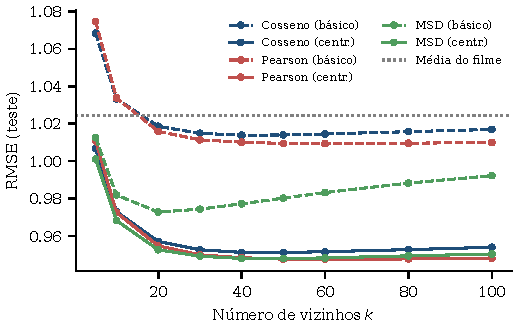
\includegraphics[width=\columnwidth]{assets/figs/fig_rmse_k.pdf}
\caption{RMSE no teste em fun\c{c}\~ao do n\'umero de vizinhos $k$ (m\'edia das 5 parti\c{c}\~oes). Linhas cont\'inuas: notas centralizadas; tracejadas: modelo b\'asico.}
\label{fig:rmsek}
\end{figure}

A centraliza\c{c}\~ao reduziu o RMSE em todas as similaridades e em todas as 5 parti\c{c}\~oes: 0,062 ponto no Pearson (de 1,009 para 0,948), 0,063 no cosseno (de 1,014 para 0,951) e 0,025 na MSD (de 0,973 para 0,948). A hip\'otese H2 foi \textbf{confirmada}: existe um $k$ intermedi\'ario \'otimo (entre 20 e 80, conforme a configura\c{c}\~ao) e a centraliza\c{c}\~ao diminui o erro. Note-se que o efeito da centraliza\c{c}\~ao \'e bem maior que o da escolha da similaridade.

\subsection{PE3: compara\c{c}\~ao com os baselines}
O KNN com Pearson centralizado atingiu RMSE de 0,948 e MAE de 0,742 (Tabela~\ref{tab:base}), contra 1,025 e 0,817 da m\'edia do filme, 1,044 e 0,836 da m\'edia do usu\'ario e 1,126 e 0,945 da m\'edia global. Isso equivale a um RMSE 7,5\% menor que o da m\'edia do filme, 9,2\% menor que o da m\'edia do usu\'ario e 15,8\% menor que o da m\'edia global, e o KNN \'e melhor em todas as 5 parti\c{c}\~oes contra os tr\^es baselines. A hip\'otese H3 foi \textbf{confirmada}, com uma ressalva sobre a magnitude: a vantagem sobre a m\'edia do filme \'e de 0,077 ponto numa escala de 1 a 5 e depende muito da centraliza\c{c}\~ao. Sem ela, o Pearson e o cosseno melhoram a m\'edia do filme em apenas 1,5\% e 1,0\% (ainda em 5 de 5 parti\c{c}\~oes), e a MSD em 5,0\%.

\begin{table}[t]
\caption{Compara\c{c}\~ao com os baselines no teste (m\'edia $\pm$ desvio padr\~ao das 5 parti\c{c}\~oes).}
\label{tab:base}
\centering
\small
\begin{tabular}{lcc}
\hline
Modelo & RMSE & MAE \\
\hline
M\'edia global & 1,126 $\pm$ 0,017 & 0,945 $\pm$ 0,015 \\
M\'edia do usu\'ario & 1,044 $\pm$ 0,012 & 0,836 $\pm$ 0,009 \\
M\'edia do filme & 1,025 $\pm$ 0,007 & 0,817 $\pm$ 0,007 \\
\textbf{KNN (Pearson, centr.)} & \textbf{0,948 $\pm$ 0,007} & \textbf{0,742 $\pm$ 0,005} \\
\hline
\end{tabular}

\end{table}

\subsection{PE4: listas de recomenda\c{c}\~ao e esparsidade}
\textit{Erro de previs\~ao por grupo.} O erro diminui com o hist\'orico do usu\'ario (Tabela~\ref{tab:groups}): o RMSE do KNN vai de 1,024 para usu\'arios com menos de 30 avalia\c{c}\~oes at\'e 0,925 para os com 120 ou mais. A vantagem sobre a m\'edia do filme tamb\'em cresce, de 4,2\% para 9,5\%.

\begin{table}[t]
\caption{RMSE no teste por n\'umero de avalia\c{c}\~oes do usu\'ario no treino (m\'edia das 5 parti\c{c}\~oes).}
\label{tab:groups}
\centering
\small
\begin{tabular}{lccc}
\hline
Avalia\c{c}\~oes & KNN & M\'edia filme & M\'edia usu\'ario \\
\hline
<30 & 1,024 & 1,068 & 1,074 \\
30-59 & 0,987 & 1,040 & 1,054 \\
60-119 & 0,936 & 1,002 & 1,031 \\
>=120 & 0,925 & 1,022 & 1,041 \\
\hline
\end{tabular}

\end{table}

\textit{Listas dos 10 filmes.} Sem restri\c{c}\~ao de vizinhos, o KNN tem Precision@10 de apenas 0,001 (Tabela~\ref{tab:topn}): ao ordenar pela nota prevista, as primeiras posi\c{c}\~oes s\~ao ocupadas por filmes pouco avaliados cuja nota vem de um \'unico vizinho. Exigir ao menos 5 vizinhos eleva a Precision@10 para 0,056, e exigir 20, para 0,093 (Recall@10 de 0,067). Mesmo assim, o KNN fica abaixo da lista dos filmes mais populares (0,157 e 0,136), e isso vale em todas as 5 parti\c{c}\~oes para o limiar de 20 (por exemplo, 0,143 contra 0,214 na primeira). O KNN s\'o supera a lista de maior nota m\'edia (0,078) com o limiar de 20.

\begin{table}[t]
\caption{Listas de 10 filmes (m\'edia $\pm$ desvio padr\~ao das 5 parti\c{c}\~oes), com o KNN Pearson centralizado.}
\label{tab:topn}
\centering
\small
\begin{tabular}{lcc}
\hline
M\'etodo & Precision@10 & Recall@10 \\
\hline
KNN ($\geq$1 vizinho) & 0,001 $\pm$ 0,000 & 0,001 $\pm$ 0,000 \\
KNN ($\geq$5 vizinhos) & 0,056 $\pm$ 0,015 & 0,036 $\pm$ 0,005 \\
KNN ($\geq$20 vizinhos) & 0,093 $\pm$ 0,029 & 0,067 $\pm$ 0,006 \\
Mais populares & 0,157 $\pm$ 0,037 & 0,136 $\pm$ 0,011 \\
Melhor m\'edia ($\geq$20 aval.) & 0,078 $\pm$ 0,026 & 0,046 $\pm$ 0,005 \\
\hline
\end{tabular}

\end{table}

A Fig.~\ref{fig:groups} mostra a Precision@10 por grupo. Ela cresce com o hist\'orico para todos os m\'etodos, inclusive os baselines, o que em parte \'e um efeito mec\^anico: usu\'arios com mais avalia\c{c}\~oes t\^em mais filmes relevantes no teste. O Recall@10 do KNN (limiar de 20) fica entre 0,057 e 0,077 em todos os grupos, sem tend\^encia de alta, enquanto o da lista dos mais populares cai (de 0,176 para 0,103). O dado mais informativo \'e a rela\c{c}\~ao entre os dois: a Precision@10 do KNN equivale a 0,49 da dos mais populares no grupo com menos de 30 avalia\c{c}\~oes e a 0,67 no grupo com 120 ou mais, ou seja, a diferen\c{c}a diminui quando h\'a mais hist\'orico.

\begin{figure}[t]
\centering
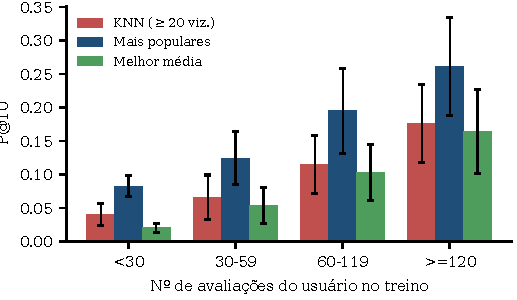
\includegraphics[width=\columnwidth]{assets/figs/fig_groups.pdf}
\caption{Precision@10 por n\'umero de avalia\c{c}\~oes do usu\'ario no treino (m\'edia e desvio padr\~ao das 5 parti\c{c}\~oes).}
\label{fig:groups}
\end{figure}

Em resumo, a hip\'otese H4 foi \textbf{parcialmente confirmada}: usu\'arios com mais avalia\c{c}\~oes recebem previs\~oes mais precisas e o KNN se aproxima mais do baseline de popularidade, mas, no protocolo adotado, as listas do KNN n\~ao acertam mais do que a lista dos filmes mais populares. Esse resultado deve ser lido com cuidado, pois a avalia\c{c}\~ao offline s\'o considera relevantes os filmes que o usu\'ario efetivamente avaliou, o que favorece t\'itulos populares \cite{shani2011}; ele n\~ao implica que um usu\'ario real preferiria a lista de populares.

\subsection{Suporte m\'inimo e exemplo qualitativo}
O suporte m\'inimo de 5 filmes em comum foi fixado de antem\~ao e n\~ao foi ajustado. A Tabela~\ref{tab:support} mostra que valores entre 2 e 10 d\~ao resultados pr\'oximos (0,948 a 0,952, dentro de um desvio padr\~ao), mas, a partir de 20, o erro sobe (0,964 e 0,985 com 20 e 40) e a cobertura cai de 99,7\% para 76,2\%: com exig\^encias maiores, mais pares de teste ficam sem vizinhos e recebem a m\'edia do usu\'ario, que \'e um preditor pior. Ou seja, o m\'etodo tolera bem suportes pequenos, e o custo de ser conservador demais \'e a perda de cobertura.

\begin{table}[t]
\caption{Efeito do suporte m\'inimo de filmes em comum (Pearson centralizado, com o $k$ de cada parti\c{c}\~ao).}
\label{tab:support}
\centering
\small
\begin{tabular}{lcc}
\hline
M\'inimo de filmes em comum & RMSE & Cob. (\%) \\
\hline
2 & 0,950 $\pm$ 0,007 & 99,7 \\
5 & 0,948 $\pm$ 0,007 & 99,7 \\
10 & 0,952 $\pm$ 0,006 & 98,6 \\
20 & 0,964 $\pm$ 0,006 & 91,2 \\
40 & 0,985 $\pm$ 0,008 & 76,2 \\
\hline
\end{tabular}

\end{table}

Como ilustra\c{c}\~ao, a Tabela~\ref{tab:example} mostra as recomenda\c{c}\~oes para o usu\'ario \exUser{}, cujas \exN{} avalia\c{c}\~oes correspondem \`a mediana do conjunto, com o modelo treinado em todos os dados, $k=\exK$ e ao menos 5 vizinhos. Entre os filmes que ele avaliou com nota 5 est\~ao Star Wars (1977) (5); Fargo (1996) (5); Rock, The (1996) (5); Long Kiss Goodnight, The (1996) (5); Return of the Jedi (1983) (5). As cinco recomenda\c{c}\~oes t\^em nota prevista entre 4,59 e 4,68, mas duas delas (\textit{The World of Apu} e \textit{The Gay Divorcee}) se apoiam em apenas 5 vizinhos, o m\'inimo exigido, enquanto \textit{A Close Shave} e \textit{The Shawshank Redemption} se apoiam em 80. O exemplo mostra o problema da confian\c{c}a: notas previstas altas com poucos vizinhos s\~ao menos seguras, o que \'e coerente com o desempenho fraco das listas sem restri\c{c}\~ao de vizinhos. Como o modelo foi treinado com todas as notas, n\~ao h\'a como verificar se o usu\'ario gostaria dos filmes sugeridos.

\begin{table}[t]
\caption{Recomenda\c{c}\~oes para o usu\'ario \exUser{} (KNN Pearson centralizado).}
\label{tab:example}
\centering
\footnotesize
\begin{tabular}{p{1.95in}cc}
\hline
Filme recomendado & Nota prevista & Vizinhos \\
\hline
World of Apu, The (Apur Sansar) (1959) & 4,68 & 5 \\
Gay Divorcee, The (1934) & 4,67 & 5 \\
Wallace \& Gromit: The Best of Aardman Animation (1996) & 4,62 & 47 \\
Close Shave, A (1995) & 4,61 & 80 \\
Shawshank Redemption, The (1994) & 4,59 & 80 \\
\hline
\end{tabular}

\end{table}

\subsection{Limita\c{c}\~oes}
Os resultados t\^em as seguintes limita\c{c}\~oes. (i) As 5 parti\c{c}\~oes compartilham 60\% do treino entre si, portanto n\~ao s\~ao amostras independentes e o desvio padr\~ao tende a ser subestimado; por isso a contagem de parti\c{c}\~oes em que um m\'etodo vence foi usada como apoio, e n\~ao foi feito teste estat\'istico formal. (ii) A varia\c{c}\~ao entre parti\c{c}\~oes \'e grande nas listas de recomenda\c{c}\~ao (desvio padr\~ao de 0,029 na Precision@10 do KNN), em parte porque as divis\~oes n\~ao s\~ao estratificadas por usu\'ario. (iii) A avalia\c{c}\~ao \'e offline e favorece itens populares. (iv) A grade de $k$ vai at\'e 100, mas as curvas s\~ao planas nessa regi\~ao e n\~ao indicam ganho al\'em dela. (v) Os dados s\~ao de 1997 e 1998 e todos os usu\'arios t\^em ao menos 20 notas. (vi) N\~ao foram comparados m\'etodos item-item nem de fatora\c{c}\~ao matricial.

%=====================================================================
\section{Conclus\~ao}
Este trabalho avaliou a filtragem colaborativa baseada em usu\'arios com KNN no MovieLens 100K. Respondendo \`a pergunta principal, as notas de usu\'arios com gostos semelhantes de fato ajudam a prever o que um usu\'ario avaliaria: o melhor modelo (Pearson com notas centralizadas, em torno de 40 a 80 vizinhos) obteve RMSE de 0,948, 7,5\% menor que o da m\'edia por filme, e superou todos os baselines em todas as parti\c{c}\~oes. O maior ganho veio da centraliza\c{c}\~ao das notas e n\~ao da escolha da similaridade: com a centraliza\c{c}\~ao, Pearson e MSD empataram e superaram levemente o cosseno, e sem ela a MSD foi a melhor.

Das quatro hip\'oteses, uma foi refutada (H1), duas foram confirmadas (H2 e H3) e uma foi parcialmente confirmada (H4). O erro de previs\~ao diminuiu com o hist\'orico do usu\'ario, mas, nas listas dos 10 filmes mais recomendados, o KNN ficou abaixo da lista dos filmes mais populares (Precision@10 de 0,093 contra 0,157), e s\'o passou a ser competitivo com os baselines de nota m\'edia ao exigir um n\'umero m\'inimo de vizinhos, o que mostra a import\^ancia de considerar a confian\c{c}a da previs\~ao ao ordenar recomenda\c{c}\~oes.

Como trabalhos futuros, sugerem-se: comparar com o KNN item-item e com fatora\c{c}\~ao matricial; combinar o KNN com a popularidade em um modelo h\'ibrido; avaliar m\'etricas al\'em da acur\'acia, como diversidade e novidade; usar conjuntos mais recentes e maiores; e aplicar testes estat\'isticos adequados \`a depend\^encia entre as parti\c{c}\~oes.

%=====================================================================
\begin{thebibliography}{00}
\bibitem{resnick1994} P. Resnick, N. Iacovou, M. Suchak, P. Bergstrom, and J. Riedl, ``GroupLens: An open architecture for collaborative filtering of netnews,'' in \textit{Proc. ACM Conf. Comput. Supported Cooperative Work (CSCW)}, Chapel Hill, NC, USA, 1994, pp. 175--186.
\bibitem{desrosiers2011} C. Desrosiers and G. Karypis, ``A comprehensive survey of neighborhood-based recommendation methods,'' in \textit{Recommender Systems Handbook}, F. Ricci, L. Rokach, B. Shapira, and P. B. Kantor, Eds. Boston, MA, USA: Springer, 2011, pp. 107--144.
\bibitem{herlocker1999} J. L. Herlocker, J. A. Konstan, A. Borchers, and J. Riedl, ``An algorithmic framework for performing collaborative filtering,'' in \textit{Proc. 22nd Annu. Int. ACM SIGIR Conf. Res. Develop. Inf. Retrieval}, Berkeley, CA, USA, 1999, pp. 230--237.
\bibitem{harper2015} F. M. Harper and J. A. Konstan, ``The MovieLens datasets: History and context,'' \textit{ACM Trans. Interact. Intell. Syst.}, vol. 5, no. 4, Art. no. 19, Dec. 2015, doi: 10.1145/2827872.
\bibitem{hug2020} N. Hug, ``Surprise: A Python library for recommender systems,'' \textit{J. Open Source Softw.}, vol. 5, no. 52, Art. no. 2174, 2020, doi: 10.21105/joss.02174.
\bibitem{sarwar2001} B. Sarwar, G. Karypis, J. Konstan, and J. Riedl, ``Item-based collaborative filtering recommendation algorithms,'' in \textit{Proc. 10th Int. Conf. World Wide Web (WWW)}, Hong Kong, 2001, pp. 285--295.
\bibitem{grouplens} GroupLens Research, ``MovieLens 100K dataset.'' Accessed: Nov. 2026. [Online]. Available: https://grouplens.org/datasets/movielens/100k/
\bibitem{harris2020} C. R. Harris \textit{et al.}, ``Array programming with NumPy,'' \textit{Nature}, vol. 585, no. 7825, pp. 357--362, Sep. 2020, doi: 10.1038/s41586-020-2649-2.
\bibitem{hunter2007} J. D. Hunter, ``Matplotlib: A 2D graphics environment,'' \textit{Comput. Sci. Eng.}, vol. 9, no. 3, pp. 90--95, 2007.
\bibitem{shani2011} G. Shani and A. Gunawardana, ``Evaluating recommendation systems,'' in \textit{Recommender Systems Handbook}, F. Ricci, L. Rokach, B. Shapira, and P. B. Kantor, Eds. Boston, MA, USA: Springer, 2011, pp. 257--297.
\end{thebibliography}

\end{document}
